\documentclass[12pt]{article}
\usepackage[letterpaper,margin=0.7in,headheight=15pt,headsep=16pt,footskip=25pt]{geometry}
\usepackage{tikz,array,fancyhdr,lmodern}
\renewcommand{\familydefault}{\sfdefault}
\pagestyle{fancy}\fancyhf{}\renewcommand{\headrulewidth}{0.35pt}
\fancyhead[L]{\small Week 26 / Same area, different boundaries encore / Grades K--5}
\fancyfoot[L]{\scriptsize Bellingham Math Circle / Week 26 / W26-BON-v1}\fancyfoot[R]{\scriptsize\thepage}
\setlength{\parindent}{0pt}\setlength{\parskip}{9pt}
\newcommand{\problem}[2]{\par\textbf{Problem #1:} #2\par}
\newcommand{\lines}[1]{\foreach \y in {1,...,#1}{\par\vspace{20pt}\hrule height 0.3pt\relax}}
\newcommand{\squaregrid}{\begin{tikzpicture}[x=2cm,y=2cm]\draw[step=1,gray!70] (0,0) grid (4,4);\end{tikzpicture}}
\newcommand{\poly}[2]{\begin{tikzpicture}[x=0.8cm,y=0.8cm]\foreach \x/\y in {#2}\draw[fill=gray!12] (\x,\y) rectangle ++(1,1);\node[anchor=north west] at (0,-0.2){#1};\end{tikzpicture}}
\newcommand{\recordgrid}{\begin{tikzpicture}[x=1.2cm,y=1.2cm]\draw[step=1,gray!70] (0,0) grid (2,2);\end{tikzpicture}}
\begin{document}
\problem{1}{Fill a 4 $\times$ 4 square with eight R tiles and eight B tiles. Each room must be joined through tile sides. Make the shared fence between the rooms as short as possible. Count one unit for each tile side.}
\vspace{10pt}
\squaregrid\hfill\squaregrid
\vspace{8pt}
\begin{tabular}{|p{1.5in}|p{1.5in}|p{1.5in}|}\hline R boundary&B boundary&Shared fence\\\hline\rule{0pt}{33pt}&&\\\hline\rule{0pt}{33pt}&&\\\hline\end{tabular}
\vspace{12pt}
\problem{2}{Keep the same 4 $\times$ 4 square. Try several divisions into two rooms. Find a rule connecting the two room-boundary lengths, the shared fence, and the outside boundary of the square.}
\lines{6}
\newpage
For these shapes, tiles must join through sides. At every grid corner, forbid the two-diagonal-tile pattern shown crossed out, even if those tiles connect elsewhere. Count corners on every boundary, including holes.
\begin{center}
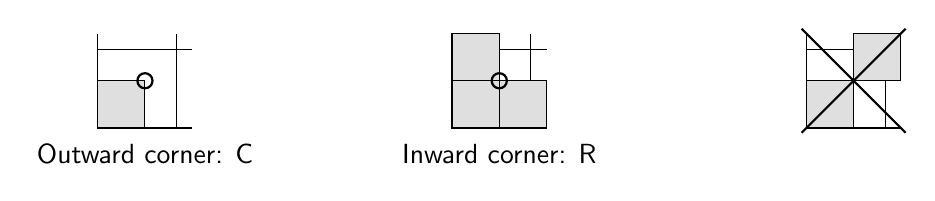
\begin{tikzpicture}[x=0.6cm,y=0.6cm]
\draw[fill=gray!25] (0,0) rectangle (1,1);\draw (0,0) grid (2,2);\draw[thick] (1,1) circle (0.16);\node at (1,-0.55){Outward corner: C};
\begin{scope}[xshift=4.5cm]\draw (0,0) grid (2,2);\foreach \x/\y in {0/0,0/1,1/0}\draw[fill=gray!25] (\x,\y) rectangle ++(1,1);\draw[thick] (1,1) circle (0.16);\node at (1,-0.55){Inward corner: R};\end{scope}
\begin{scope}[xshift=9cm]\draw (0,0) grid (2,2);\foreach \x/\y in {0/0,1/1}\draw[fill=gray!25] (\x,\y) rectangle ++(1,1);\draw[thick] (-0.1,-0.1)--(2.1,2.1) (-0.1,2.1)--(2.1,-0.1);\end{scope}
\end{tikzpicture}
\end{center}
\problem{3}{Build these shapes. Count their outward corners C, inward corners R, and holes. What rule connects the three counts?}
\begin{center}
\poly{1}{0/0,1/0,2/0,0/1,1/1,2/1}\hspace{2cm}\poly{2}{0/0,1/0,2/0,0/1,0/2}
\par\vspace{12pt}
\poly{3}{0/0,1/0,2/0,0/1,2/1,0/2,1/2,2/2}\hspace{1cm}\poly{4}{0/0,1/0,2/0,3/0,4/0,0/1,2/1,4/1,0/2,1/2,2/2,3/2,4/2}
\end{center}
\begin{tabular}{|p{0.65in}|p{1in}|p{1in}|p{1in}|}\hline Shape&C&R&Holes\\\hline\rule{0pt}{27pt}1&&&\\\hline\rule{0pt}{27pt}2&&&\\\hline\rule{0pt}{27pt}3&&&\\\hline\rule{0pt}{27pt}4&&&\\\hline\end{tabular}
\lines{2}
\newpage
Each footprint square supports the stated number of cubes in a solid vertical stack. Faces where cubes touch are covered. Count all other faces, including the bottom.
\begin{center}
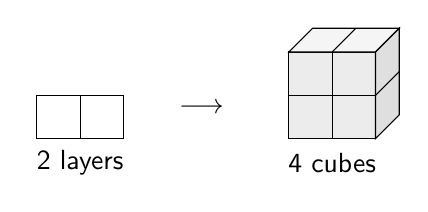
\begin{tikzpicture}[x=0.55cm,y=0.55cm]
\draw[step=1] (0,0) grid (2,1);\node at (1,-0.55){2 layers};
\node at (3.8,0.7){$\longrightarrow$};
\begin{scope}[xshift=3.2cm]\draw[fill=gray!15] (0,0) rectangle (2,2);\draw (1,0)--(1,2) (0,1)--(2,1);\draw[fill=gray!8] (0,2)--(.55,2.55)--(2.55,2.55)--(2,2)--cycle;\draw (1,2)--(1.55,2.55);\draw[fill=gray!25] (2,0)--(2.55,.55)--(2.55,2.55)--(2,2)--cycle;\draw (2,1)--(2.55,1.55);\node at (1,-0.55){4 cubes};\end{scope}
\end{tikzpicture}
\end{center}
\problem{4}{Build each of these three buildings with eight cubes. Count every exposed square face. Which building has the least exposed surface?}
\begin{center}
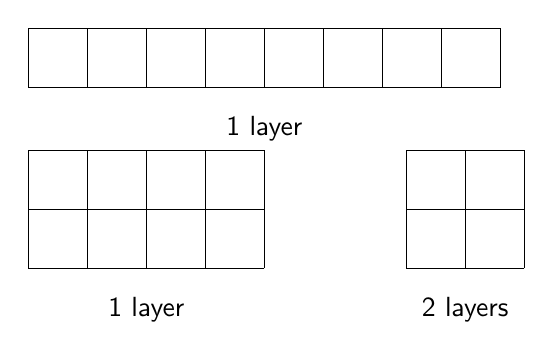
\begin{tikzpicture}[x=0.75cm,y=0.75cm]
\draw[step=1] (0,0) grid (8,1);\node at (4,-0.7){1 layer};
\begin{scope}[yshift=-2.3cm]\draw[step=1] (0,0) grid (4,2);\node at (2,-0.7){1 layer};\end{scope}
\begin{scope}[xshift=4.8cm,yshift=-2.3cm]\draw[step=1] (0,0) grid (2,2);\node at (1,-0.7){2 layers};\end{scope}
\end{tikzpicture}
\end{center}
\begin{tabular}{|p{1.75in}|p{1.75in}|p{1.75in}|}\hline Row of eight&2 $\times$ 4, one layer&2 $\times$ 2, two layers\\\hline\rule{0pt}{44pt}&&\\\hline\end{tabular}
\vspace{12pt}
\problem{5}{Make a building with equal-height stacks on every square of a footprint. How can the footprint's area, its boundary length, and the number of layers tell you the exposed-face count? Find a rule that works for footprints with holes too.}
\lines{7}
\newpage
\problem{6}{Use a 2 $\times$ 2 footprint. Put stacks of heights 1, 2, 3, and 4 on its four squares, using each height once. Arrange them to make the fewest exposed faces, and then the most.}
\vspace{8pt}
\recordgrid\hfill\recordgrid\hfill\recordgrid
\par\vspace{18pt}
\recordgrid\hfill\recordgrid\hfill\recordgrid
\vspace{16pt}
\lines{6}
\end{document}
